\begin{frame}[t]{Datennahme}

  \begin{columns}[t,onlytextwidth]
    \begin{column}{0.48\textwidth}
      \begin{block}{BMP180}
        \begin{itemize}
          \item seriell
          \item Temperatur, Luftdruck
          \item 3.3V, Ground, SDA (serial data), SCL (serial clock)
        \end{itemize}
      \end{block}
    \end{column}
    %
    \begin{column}{0.48\textwidth}
      \begin{block}{DHT22}
        \begin{itemize}
          \item seriell
          \item Temperatur, Luftfeuchtigkeit
          \item 3.3V, Ground, GPIO
        \end{itemize}
      \end{block}
    \end{column}
  \end{columns}

  \begin{block}{Daten}
    \centering
    \texttt{(temp\_1, temp\_2, pressure, humidity)}
  \end{block}

\end{frame}

\begin{frame}[t]{Datennahme}
  \centering
  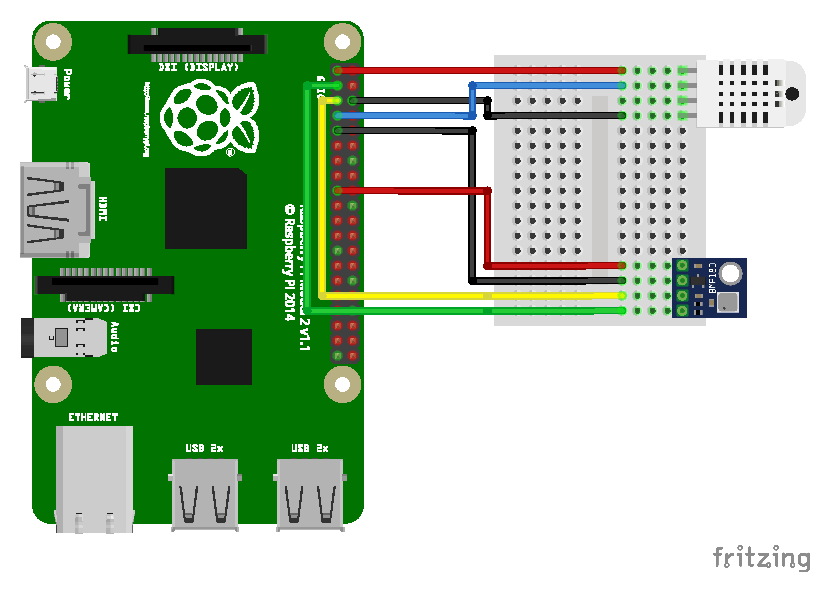
\includegraphics[width=0.8\textwidth]{../weatherstation_rpi2.pdf}
\end{frame}
